\documentclass[a0,portrait]{a0poster}
\usepackage{multicol} % multiple columns of text side-by-side
\columnsep=100pt % white space between the columns in the poster
\columnseprule=3pt % thickness of the black line between the columns in the poster

\usepackage[svgnames,dvipsnames]{xcolor} % specify colours by their names
\usepackage{tcolorbox} % coloured boxing of sections
\usepackage{tikz} % manual placement of logos
\usepackage{palatino} % use the palatino font

\usepackage{graphicx} % including images
\usepackage[font=small,labelfont=bf]{caption} % captions to tables and figures
\graphicspath{{figures/}} % location of the graphics file

\usepackage{enumitem}
\usepackage{booktabs} % top and bottom rules for table

\usepackage{amsfonts, amsmath, amsthm, amssymb} % math fonts, symbols and environments
\usepackage{wrapfig} % wrapping text around tables and figures
\usepackage{mathtools}

\begin{document}
\newcommand{\code}{\texttt}

%----------------------------------------------------------------------------------------
% title and authors
\begin{minipage}[b]{0.99\linewidth}
	\begin{center}
		\veryHuge \color{DarkRed} \textbf{Programming biological systems} \color{Black}\\ % Title
		\Huge\textit{by reverse-engineering reaction-diffusion}\\[2.4cm] % Subtitle
		\huge \textbf{Gregory Sz\'ep, Luca Cardelli, Attila Csik\'asz-Nagy}\\[0.5cm]
		\vspace{1cm}
\includegraphics[width=67cm]{abstract}
	\end{center}
\end{minipage}

% organisation logos
\begin{tikzpicture}[remember picture, overlay]
	\node [anchor=north west, inner sep=6cm]  at (-5,32) {
		
\includegraphics[height=7cm]{kcl}};
\end{tikzpicture}

\begin{tikzpicture}[remember picture, overlay]
	\node [anchor=north east, inner sep=6cm]  at (79,33) {
		
\includegraphics[height=6cm]{mrc}};
\end{tikzpicture}

\begin{tikzpicture}[remember picture, overlay]
	\node [anchor=south west, inner sep=6cm]  at (56,-88) {
		
\includegraphics[height=7cm]{epsrc}};
\end{tikzpicture}
\LARGE

% figure abstract titles
\begin{tikzpicture}[remember picture, overlay]
	\node [text width=12cm] at (14,10) {
		\begin{center}\textbf{BIOLOGICAL PROCESS}\end{center}};
\end{tikzpicture}

\begin{tikzpicture}[remember picture, overlay]
	\node [text width=12cm] at (40,12) {
		\begin{center}\textbf{DYNAMICAL SYSTEM}\end{center}};
\end{tikzpicture}

\begin{tikzpicture}[remember picture, overlay]
	\node [text width=12cm] at (66,14) {
		\begin{center}\textbf{ALGORITHM}\end{center}};
\end{tikzpicture}

% algorithm code snippet
\begin{tikzpicture}[remember picture, overlay]
	\node [text width=18cm] at (64.5,20) {
		\code{\textbf{
			for \textcolor{DarkBlue}{i} in \textcolor{DarkBlue}{set} : \\
			\qquad do \textcolor{Emerald}{this} ; \\
			\qquad if \textcolor{OliveGreen}{this} then... }}};
\end{tikzpicture}

% arrow captions
\begin{tikzpicture}[remember picture, overlay]
	\node [text width=12cm] at (25,17) {
		\begin{center}\textbf{\textcolor{Gray}{synthetic biology}}\end{center}};
\end{tikzpicture}

\begin{tikzpicture}[remember picture, overlay]
	\node [text width=10cm] at (23,26) {
		\begin{center}\textbf{\textcolor{Gray}{systems biology}}\end{center}};
\end{tikzpicture}

\begin{tikzpicture}[remember picture, overlay]
	\node [text width=10cm] at (47,28) {
		\begin{center}\textbf{\textcolor{Gray}{natural computation}}\end{center}};
\end{tikzpicture}

\vspace{-16cm}

% itemised thumbs up/down icons
\newcommand*\up{\item[{
\includegraphics[width=0.75em]{up}}\,\,]}
\newcommand*\down{\item[{
\includegraphics[width=0.75em]{down}}\,\,]}
\newcommand*\tab{\indent\indent\indent\indent\indent\indent}

%----------------------------------------------------------------------------------------
\begin{tcolorbox}[boxrule=2pt,arc=3.4pt,boxsep=2mm]
	\begin{center}
		\textbf{\color{Grey} Motivation \color{Black}$|$
		Designing algorithms to be executed in living organisms}
	\end{center}
\end{tcolorbox}
\vspace{0.25cm}

\noindent
Is it possible to build a programming language that compiles into a chemical environment,
allowing us to execute arbitrary code in living cells? To produce appropriate adaptive
responses given sensory input from environments, \textbf{living organisms perform
asynchronous computations} using chemicals reaction networks \cite{Dalchau2018ComputingClocks}.

\vspace{1cm}
\code{\textbf{\normalsize
	for \textcolor{DarkBlue}{cell} in \textcolor{DarkBlue}{lymph node} : \\
	\tab if type(\textcolor{DarkBlue}{cell}) == \textcolor{DarkRed}{"T"} : \\
	\tab\tab \textcolor{DarkBlue}{cell}.dna.append(\textcolor{Emerald}{sequence}); \\
	\tab\tab \textcolor{DarkBlue}{cell}.express(\textcolor{OliveGreen}{receptor}) \\
	\tab if \textcolor{DarkRed}{"cancerSequence"} in \textcolor{DarkBlue}{cell}.dna : \\
	\tab\tab \textcolor{DarkBlue}{cell}.init(apoptosis)
}}

\begin{tikzpicture}[remember picture, overlay]
	\node [anchor=south west, inner sep=6cm]  at (25,-5) {
		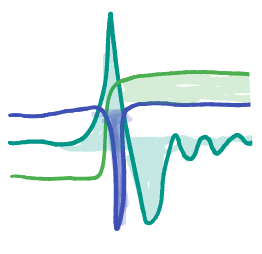
\includegraphics[height=12cm]{response-function}};
\end{tikzpicture}

\begin{tikzpicture}[remember picture, overlay]
	\node [text width=12cm] at (62,9) {
		\begin{align*}
			\partial_t\bar{\mathrm{p}}(t)=
			\!\!\!\!\!\!\!\!\!\!\!
			\overbracket[2pt][10pt]{\bar{\mathrm{R}}(\bar{\mathrm{p}}|\theta)}^{\text{reaction network}}
			\!\!\!\!\!\!\!\!\!\!\!+\!\!\!\!\!\!\!\!\!\!\!
			\underbracket[2pt][10pt]{\bar{\mathrm{S}}(t)}_{\text{sensory input}}
		\end{align*}};
\end{tikzpicture}

\begin{tikzpicture}[remember picture, overlay]
	\node [anchor=south west, inner sep=6cm]  at (15.5,2) {
		
\includegraphics[height=2cm]{rarrow}};
\end{tikzpicture}

\begin{tikzpicture}[remember picture, overlay]
	\node [text width=24cm]  at (34,15) {
		\textbf{\textcolor{Gray}{compile\\response\\function}}};
\end{tikzpicture}

\begin{tikzpicture}[remember picture, overlay]
	\node [anchor=south west, inner sep=6cm]  at (39.5,5) {
		
\includegraphics[height=2cm]{rarrow}};
\end{tikzpicture}

\begin{tikzpicture}[remember picture, overlay]
	\node [text width=24cm]  at (58,18) {
		\textbf{\textcolor{Gray}{infer\\reaction\\network}}};
\end{tikzpicture}

\vspace{-9cm}
\begin{tcolorbox}[boxrule=2pt,arc=3.4pt,boxsep=2mm]
	\begin{center}
		\textbf{\color{Grey}Leading Question \color{Black}$|$
		Given a \textit{response function} what is the \textit{minimal} reaction network?}
	\end{center}
\end{tcolorbox}

\begin{itemize}[leftmargin=3cm]
	\up Asynchronous arithmetic logic units have been designed using chemical reaction networks \cite{Cardelli2018ChemicalCircuits.}
	\up Chemical reaction networks can be inferred from processes
	data \cite{Galagali2016BayesianNetworks}
	\down No mapping between response function and network exists that minimises complexity
\end{itemize}



%----------------------------------------------------------------------------------------
\begin{multicols}{2}

\begin{tcolorbox}[boxrule=2pt,arc=3.4pt,boxsep=2mm]
	\begin{center}
		\textbf{
		What is the general routine for \textit{reducing complexity} in reaction networks?}
	\end{center}
\end{tcolorbox}

\begin{itemize}[leftmargin=3cm]
	\up For \textit{known time-scale separations} one can reduce models, introducing memory effects~\cite{Phillies2000ProjectionFormalism}
	\down There exist no \textit{unsupervised reduction} methods\\beyond
	empirical sensitivity analysis
\end{itemize}

\vfill
\columnbreak

\begin{tcolorbox}[boxrule=2pt,arc=3.4pt,boxsep=2mm]
	\begin{center}
		\textbf{
		How does evolution lead to \textit{complexity increase} in network motifs such as switches and clocks?}
	\end{center}
\end{tcolorbox}

\begin{itemize}[leftmargin=3cm]
	\up Relationship between robustness and \\evolvability has been investigated \cite{Daniels2008SloppinessBiology}
	\down Evolutionary relationships between different chemical networks have not been quantified
\end{itemize}

\vfill
\end{multicols}
\vspace{1cm}
%----------------------------------------------------------------------------------------

\begin{tcolorbox}[boxrule=2pt,arc=3.4pt,boxsep=2mm]
	\begin{center}
		\textbf{\color{Grey}Follow-up Question \color{Black}$|$
		Given a \textit{steady state pattern} what is the \textit{minimal} reaction-diffusion network?}
	\end{center}
\end{tcolorbox}

\begin{itemize}[leftmargin=3cm]
	\up Dynamics of local equilibria show promising pattern formation analysis beyond linear stability \cite{Halatek2018}
	\down No geometric description of diffusive attractors in phase space exists; required for pattern design
\end{itemize}

\begin{tikzpicture}[remember picture, overlay]
	\node [anchor=south west, inner sep=6cm]  at (-3,-17) {
		
\includegraphics[height=12cm]{pattern}};
\end{tikzpicture}

\begin{tikzpicture}[remember picture, overlay]
	\node [anchor=south west, inner sep=6cm]  at (22,-15) {
		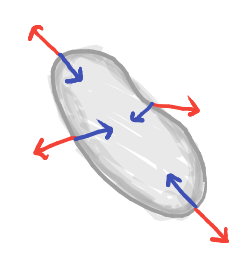
\includegraphics[height=12cm]{geometrisation}};
\end{tikzpicture}

\begin{tikzpicture}[remember picture, overlay]
	\node [text width=12cm] at (56,-2) {
		\begin{align*}
			\partial_t\bar{\mathrm{p}}(\bar{\mathrm{x}},t)=
			\!\!\!\!\!\!\!\!\!\!\!
			\overbracket[2pt][10pt]{\bar{\mathrm{R}}(\bar{\mathrm{p}}|\theta)}^{\text{reaction network}}
			\!\!\!\!\!\!\!\!\!\!\!+D
			\underbracket[2pt][10pt]{\partial_{\bar{\mathrm{x}}}^2\,
			\bar{\mathrm{p}}(\bar{\mathrm{x}},t)}_{\text{diffusion}}
		\end{align*}};
\end{tikzpicture}

\begin{tikzpicture}[remember picture, overlay]
	\node [anchor=south west, inner sep=6cm]  at (12,-6) {
		
\includegraphics[height=2cm]{rarrow}};
\end{tikzpicture}

\begin{tikzpicture}[remember picture, overlay]
	\node [text width=24cm]  at (29,1) {
		\textbf{\textcolor{Gray}{geometrisation}}};
\end{tikzpicture}

\begin{tikzpicture}[remember picture, overlay]
	\node [anchor=south west, inner sep=6cm]  at (35,-2) {
		
\includegraphics[height=2cm]{rarrow}};
\end{tikzpicture}

\begin{tikzpicture}[remember picture, overlay]
	\node [text width=24cm]  at (54,5) {
		\textbf{\textcolor{Gray}{inference}}};
\end{tikzpicture}

\begin{tikzpicture}[remember picture, overlay]
	\node [text width=12cm] at (31,7) {
		\begin{align*}\textcolor{red}{\bar{\mathrm{R}}}\end{align*}};
\end{tikzpicture}

\begin{tikzpicture}[remember picture, overlay]
	\node [text width=12cm] at (33.5,9.75) {
		\begin{align*}\textcolor{DarkBlue}{D}\end{align*}};
\end{tikzpicture}

%----------------------------------------------------------------------------------------
\vspace{-1cm}
\vfill\normalsize

\begin{minipage}[t][][b]{0.99\textwidth}
	\bibliographystyle{style}
	\bibliography{mendeley_v2}
\end{minipage}

\end{document}
